\externaldocument{tech_eclipse_text}

\section{Set-up and Terminology \label{terminology}}
The eclipse mapping program described in this paper derives a model for the relative surface brightness of a transiting planet host star when given a single band, short cadence light curve of the target as an input.  Each run of the program produces a static surface map. By applying the code to a series of short segments of the light curve, we are able to derive a model for the time evolution of the star's surface brightness.  

The stellar rotation period, $P_{rot}$, is an input parameter into the program along with the orbital and physical properties of the planet, including the
planet radius relative to the host star, $R_{p}$, the orbital period, $P_{orb}$, etc.   **OTHER INPUTS Need defining?**
The star is assumed to be rotating as a uniform solid body.  In addition, we require the spin-axis of the star   
to be aligned with the orbital axis of the planet and the planet to be on a circular orbit.  
%These criteria are both met for our test object, Kepler-17 \cite{}.  }

In order to efficiently {\bf describe the details of our program}, the geometry
of the problem must be defined and some basic terminology must be established.
We divide the stellar surface into a series of large {\it regions}, as shown in Figure~\ref{fig:CoRoT}.  
While describing our program in this paper, the regions along the line of transit will be called {\it boxes}; 
the total longitudinal regions will be called {\it longitudes};
and the longitudinal regions with the box areas subtracted will be referred to as {\it stripes}.
When talked about as an ensemble or when the distinction is unimportant, these regions will be referred to as just that - {\it regions}. 

++++STOPPED HERE++++

Typically, 
%causing the regions to rotate in and out of view over time.  
The surface brightness, $b_j$, of
each region is held constant 

longitudinal stripes. Additionally, we add a set of boxes that lie along the path of the eclipsing planet

\begin{figure}[h]
	\centering
	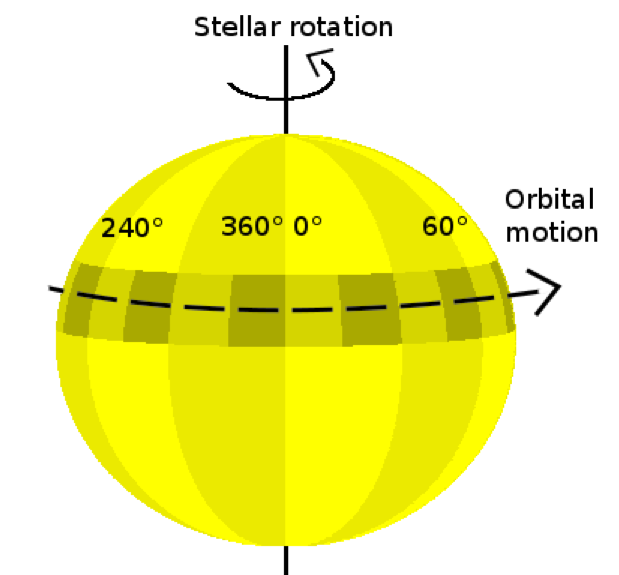
\includegraphics[width=.5\textwidth]{images/modelGeometry.png}
	\caption{CoRoT brightness map.}
	\label{CoRoT}
\end{figure}


Our program calculates the model flux at each time step, by summing over the surface of the visible sphere according to:

\begin{equation}
	\fmod = \sum_j V_{i,j}b_j, 
\end{equation}

where $b_j$ is the brightness per unit area for region $j$ and $V_{i,j}$ is the {\it visibility} of that region at time, $i$.


This model flux has two parts: a visibility and a brightness value. The amoeba determines the brightness values while the visibility values are pre-defined. Both of these apply to a set of $j$ regions. 
The planet will occlude only the boxes and will do so only during a transit. The longitudes' brightness values are defined as:

\begin{equation}
Z_j = \frac{S_j - \frac{c}{q} \sum_{j=1}^{q}B_j}{1- c}
\end{equation}

Where $q$ is the ratio of $n_{boxes}$ to $n_{stripes}$ and $c$ is the ratio of the total eclipsed area to the non-eclipsed area. $c$ can be calculated by the same set of integrals that will be used for the visibilities.

If the Amoeba algorithm is given the set of boxes and stripes, they will be able to vary to offset each other creating a "zebra" pattern in the brightness map.  The longitude values create parameter independence by warping the chi-squared space so that such a case is less likely to become a local minimum. The Amoeba algorithm takes the set of box brightness guesses and longitude brightness guesses as inputs. During each call of the chi-squared algorithm the stripe values are calculated from the longitudes and boxes. The boxes and the stripes are then used to calculate the model flux.

